The FESTIM code was compared to TMAP7 \sidecite{longhurst_tmap7_2008} on a 1D case.

The 1D simulation case is a \SI{8.5}{mm}-thick composite slab made of W, Cu and CuCrZr (see \reffig{monoblock 1D geometry}).
The plasma facing surface $\Gamma_\mathrm{top}$ is located at $x=\SI{0}{mm}$ and the surface cooled by water $\Gamma_\mathrm{coolant}$ is located at $x=\SI{8.5}{mm}$.
The trapping parameters are detailed in \reftab{traps comparison tmap}.
The boundary conditions are detailed in \refeq{code comparison BCs}.

\begin{figure}
    \begin{overpic}[width=0.75\linewidth]{Figures/Chapter3/monoblocks/interface_condition/iter case/Monoblock 1D.pdf}
        \put(40, 50){\SI{6}{mm}}
        \put(40, 8){W}
        \put(62, 50){\SI{1}{mm}}
        \put(65, 8){Cu}
        \put(72, 50){\SI{1.5}{mm}}
        \put(72, 8){CuCrZr}
        \put(6, 25){\large$\Gamma_\mathrm{top}$}
        \put(85, 25){\large$\Gamma_\mathrm{coolant}$}
    \end{overpic}
    \caption{TMAP7 - FESTIM comparison 1D geometry showing W \cruleme[grey]{0.3cm}{0.3cm}, Cu \cruleme[orange]{0.3cm}{0.3cm}, CuCrZr \cruleme[yellow]{0.3cm}{0.3cm}}
    \labfig{monoblock 1D geometry}
\end{figure}

\begin{table*}
    \centering
    \begin{tabular}{L{1.5cm} L{1.5cm} R{1.7cm} R{1.1cm} R{1.6cm} R{1.1cm} R{1.9cm}}
         & Material & $k_0 (\si{m^3.s^{-1}})$ &  $E_k (\si{eV})$ & $p_0 (\si{s^{-1}})$ & $E_p (\si{eV})$ & $n_i (\si{at.fr.})$ \\
        \hline
        \\
        Trap 1 & W & $3.8 \times 10^{-17}$ & 0.39 & $8.4 \times 10^{12}$& 1.20 & $5.0 \times 10^{-4}$ \\
        \\
        Trap 2 & W & $3.8 \times 10^{-17}$ & 0.39 & $8.4 \times 10^{12}$& 1.40 & $5.0 \times 10^{-3}$ \\
        \\
        Trap 3 & Cu & $6.0 \times 10^{-17}$ & 0.39 & $8.0 \times 10^{13}$ & 0.50 &$5.0 \times 10^{-5}$\\
        \\
        Trap 4 & CuCrZr & $1.2\times 10^{-16}$ & 0.42 & $8.0 \times 10^{13}$ & 0.50 &$5.0 \times 10^{-5}$\\
        \\
        Trap 5 & CuCrZr & $1.2\times 10^{-16}$ & 0.42 & $8.0 \times 10^{13}$ & 0.83 &$4.0 \times 10^{-2}$\\
        \\
    \end{tabular}
    \caption{Traps properties used in the comparison with TMAP7.}
    \labtab{traps comparison tmap}
\end{table*}

\begin{subequations}
    \begin{align}
    T &= \SI{1200}{K}\quad \text { on } \Gamma_\mathrm{top}\\
    c_\mathrm{m} &=  \frac{\varphi_\mathrm{imp} \cdot R_p}{D} \quad \text { on } \Gamma_\mathrm{top}\\
    T &= \SI{373}{K} \quad \text { on } \Gamma_\mathrm{coolant}\\
    -D \nabla c_\mathrm{m} \cdot \mathbf{n} &= K_\mathrm{CuCrZr} \cdot c_\mathrm{m}^{2} \quad \text { on } \Gamma_\mathrm{coolant}  
    \end{align}
    \labeq{code comparison BCs}
\end{subequations}
with $\varphi_\mathrm{imp} = \SI{5e23}{m^{-2}.s^{-1}}$ the implanted particle flux, $R_p = \SI{1.25}{nm}$ the implantation depth, $\mathbf{n}$ the normal vector and $K_\mathrm{CuCrZr} = 2.9 \times 10^{-14}\cdot \exp{(-1.92/(k_B\cdot T))}$ the recombination coefficient of the CuCrZr (in vacuum) expressed in \si{m^4.s^{-1}} \sidecite{anderl_deuterium_1999}.

The Dirichlet boundary condition on $\Gamma_\mathrm{top}$ for the hydrogen transport corresponds to a flux balance between the implanted flux and the flux that is retro-desorbed at the surface (see Section \ref{triangle model}).
The temperature profile in TMAP7 was fixed on the temperature profile produced by FESTIM (see \reffig{temperature}).

TMAP7 and FESTIM were found to be in very good agreement (see \reffig{code comparison}).

\begin{figure*} [h]
    \centering
    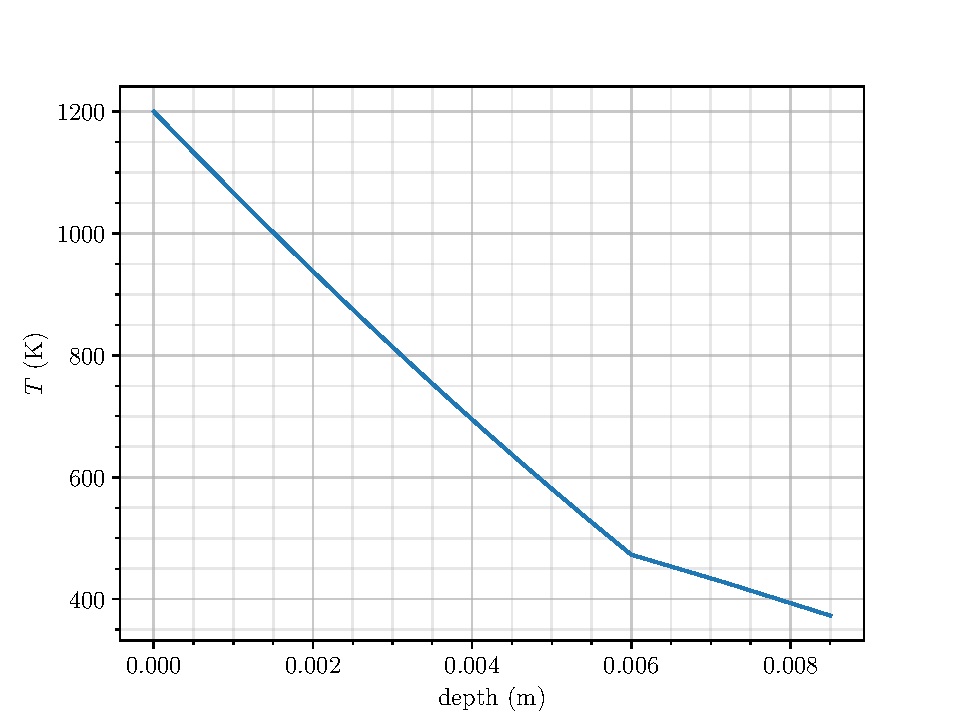
\includegraphics[width=0.5\linewidth]{Figures/Chapter3/monoblocks/interface_condition/iter case/temperature_1D.pdf}
    \caption{Temperature profile simulated by FESTIM for comparison case with TMAP7.}
    \labfig{temperature}
\end{figure*}

\begin{figure} [h]
    \centering
    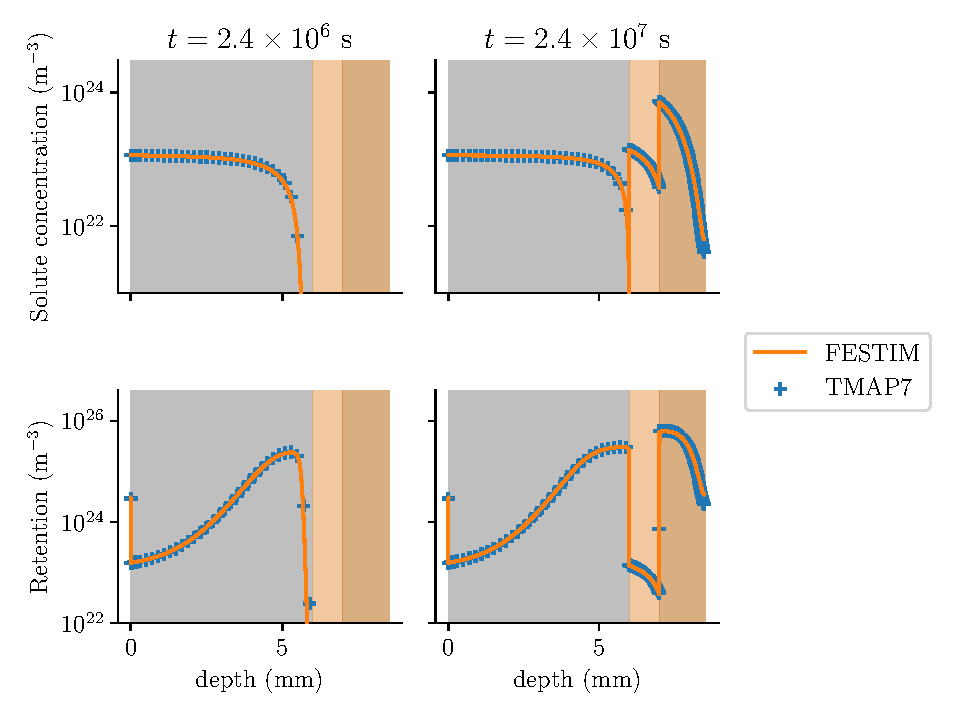
\includegraphics[width=\linewidth]{Figures/Chapter3/monoblocks/interface_condition/iter case/comparison_codes.pdf}
    \caption{Comparison of results provided by FESTIM and TMAP7}
    \labfig{code comparison}
\end{figure}

